\documentclass[12pt, a4paper]{article}
\usepackage[margin=1in]{geometry}
\usepackage{amsmath}
\usepackage{amssymb}
\usepackage{graphicx}
\usepackage{hyperref}
\usepackage{tikz}
\usetikzlibrary{decorations.pathmorphing} % For drawing photons
\usepackage{siunitx} % For SI units
\usepackage{caption} % For better figure captioning

\title{Bohr Model: New Practice Problems and Solutions}
\author{}
\date{\today}

\begin{document}
\maketitle

\section*{New Practice Problems}
\hrulefill

\subsection*{Problem 1: Recoil of an Ion}
\begin{quote}
A doubly ionized lithium atom (Li$^{2+}$, Z=3) is at rest in its first excited state (n=2). It de-excites to the ground state (n=1) by emitting a single photon. Calculate the recoil velocity of the ion. [Mass of a lithium ion is approximately $1.15 \times 10^{-26}$ kg]
\end{quote}

\textbf{Explanation \& Solution:}
\begin{enumerate}
    \item \textbf{Calculate the Photon's Energy:} The energy levels for a hydrogen-like ion are given by $E_n = -13.6 \frac{Z^2}{n^2}$ eV. For Li$^{2+}$, Z=3.
    \begin{itemize}
        \item Initial energy (n=2): $E_2 = -13.6 \frac{3^2}{2^2} = -30.6$ eV.
        \item Final energy (n=1): $E_1 = -13.6 \frac{3^2}{1^2} = -122.4$ eV.
        \item Photon energy: $E_{\gamma} = |E_1 - E_2| = |-122.4 - (-30.6)| = 91.8$ eV.
    \end{itemize}

    \item \textbf{Calculate the Photon's Momentum:} First, convert energy to Joules.
    \begin{itemize}
        \item $E_{\gamma} = 91.8 \text{ eV} \times (1.602 \times 10^{-19} \text{ J/eV}) \approx 1.47 \times 10^{-17}$ J.
        \item $p_{\gamma} = \frac{E_{\gamma}}{c} = \frac{1.47 \times 10^{-17} \text{ J}}{3.0 \times 10^8 \text{ m/s}} \approx 4.90 \times 10^{-26}$ kg$\cdot$m/s.
    \end{itemize}

    \item \textbf{Apply Momentum Conservation:} The recoil momentum of the ion, $p_{ion}$, must be equal in magnitude to the photon's momentum.
    $$ p_{ion} = p_{\gamma} = 4.90 \times 10^{-26} \text{ kg}\cdot\text{m/s} $$

    \item \textbf{Calculate Recoil Velocity:}
    $$ v_{recoil} = \frac{p_{ion}}{m_{Li}} = \frac{4.90 \times 10^{-26} \text{ kg m/s}}{1.15 \times 10^{-26} \text{ kg}} \approx 4.26 \text{ m/s} $$
\end{enumerate}
\textbf{Final Answer:} The recoil velocity of the lithium ion is approximately \textbf{4.26 m/s}.

\hrulefill
\subsection*{Problem 2: Multi-Photon Emission After Collision}
\begin{quote}
A hydrogen atom, initially in its ground state (n=1), absorbs a photon and is excited. It then de-excites back to the ground state by emitting two photons in sequence. The second photon emitted has an energy of 1.89 eV.
(a) To which energy level (n) was the atom initially excited?
(b) What was the wavelength of the original incident photon that caused the excitation?
\end{quote}

\begin{figure}[h!]
\centering
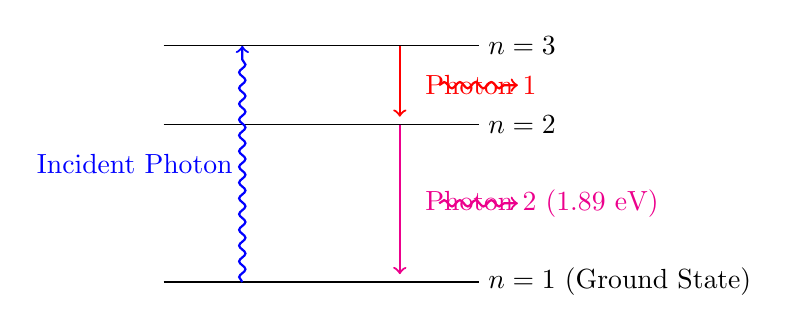
\begin{tikzpicture}
    % Energy levels
    \draw (-2,0) -- (2,0) node[right]{$n=1$ (Ground State)};
    \draw (-2,2) -- (2,2) node[right]{$n=2$};
    \draw (-2,3) -- (2,3) node[right]{$n=3$};
    
    % Excitation
    \draw[->, thick, blue, decorate, decoration={snake,amplitude=0.4mm,segment length=2mm,post length=1mm}] (-1,0) -- (-1,3);
    \node[left, blue] at (-1, 1.5) {Incident Photon};
    
    % De-excitation cascade
    \draw[->, thick, red] (1,3) -- (1,2.1);
    \node[right, red] at (1.2, 2.5) {Photon 1};
    \draw[->, thick, red, decorate, decoration={snake,amplitude=0.4mm,segment length=2mm,post length=1mm}] (1.5, 2.5) -- (2.5, 2.5);
    
    \draw[->, thick, magenta] (1,2) -- (1,0.1);
    \node[right, magenta] at (1.2, 1) {Photon 2 (1.89 eV)};
    \draw[->, thick, magenta, decorate, decoration={snake,amplitude=0.4mm,segment length=2mm,post length=1mm}] (1.5, 1) -- (2.5, 1);
\end{tikzpicture}
\caption{Energy level diagram for Problem 2.}
\end{figure}

\textbf{Solution:}
\begin{description}
    \item[(a) Determine the Energy Levels:] The second emitted photon (1.89 eV) corresponds to the transition from $n=3$ to $n=2$. Since this was the second photon in a cascade down to the ground state ($n=1$), the full de-excitation path must have been $3 \to 2 \to 1$. Therefore, the atom was initially excited to the \textbf{n=3 level}.

    \item[(b) Calculate Incident Photon Wavelength:] The incident photon caused the excitation from $n=1$ to $n=3$.
    \begin{itemize}
        \item Energy required: $\Delta E_{1 \to 3} = E_3 - E_1 = \left(-\frac{13.6}{3^2}\right) - \left(-\frac{13.6}{1^2}\right) \approx 12.09$ eV.
        \item Wavelength: $\lambda = \frac{hc}{E} = \frac{1240 \text{ eV}\cdot\text{nm}}{12.09 \text{ eV}} \approx 102.6$ nm.
    \end{itemize}
\end{description}
\textbf{Final Answers:} (a) The atom was excited to the \textbf{n=3} level. (b) The wavelength of the incident photon was \textbf{102.6 nm}.


\hrulefill
\subsection*{Problem 3: Excitation by Collision and Possible Emissions}
\begin{quote}
A stationary singly ionized helium ion (He$^{+}$) is in a state with orbital angular momentum $L = \frac{h}{\pi}$. It is struck by a proton with 50 eV of kinetic energy. Assuming the proton can transfer all or part of its energy, what are the possible wavelengths of light that can be emitted as the ion de-excites?
\end{quote}

\textbf{Solution:}
\begin{enumerate}
    \item \textbf{Determine the Initial State:} Given $L = n \frac{h}{2\pi}$, an angular momentum of $L = \frac{h}{\pi}$ implies the ion starts in the \textbf{n=2} state.

    \item \textbf{Identify Possible Excitations:} The proton's 50 eV energy is available. The ionization energy of He$^{+}$ from the n=2 state is $E_{\infty} - E_2 = 0 - (-\frac{54.4}{2^2}) = 13.6$ eV. Since 50 eV > 13.6 eV, the proton has enough energy to excite the ion to any higher level.

    \item \textbf{Determine Possible Emission Wavelengths:} We calculate the wavelengths for several key de-excitation pathways.
    \begin{itemize}
        \item Transition $4 \to 3$: $\Delta E = 54.4(\frac{1}{3^2}-\frac{1}{4^2}) \approx 2.64$ eV $\implies \lambda \approx \textbf{469 nm}$.
        \item Transition $4 \to 2$: $\Delta E = 54.4(\frac{1}{2^2}-\frac{1}{4^2}) = 10.2$ eV $\implies \lambda \approx \textbf{121.6 nm}$.
        \item Transition $3 \to 2$: $\Delta E = 54.4(\frac{1}{2^2}-\frac{1}{3^2}) \approx 7.56$ eV $\implies \lambda \approx \textbf{164 nm}$.
        \item Transition $3 \to 1$: $\Delta E = 54.4(\frac{1}{1^2}-\frac{1}{3^2}) \approx 48.36$ eV $\implies \lambda \approx \textbf{25.6 nm}$.
        \item Transition $2 \to 1$: $\Delta E = 54.4(\frac{1}{1^2}-\frac{1}{2^2}) = 40.8$ eV $\implies \lambda \approx \textbf{30.4 nm}$.
    \end{itemize}
\end{enumerate}
\textbf{Final Answer:} Prominent possible wavelengths are \textbf{469 nm, 164 nm, 121.6 nm, 30.4 nm, and 25.6 nm}.

\hrulefill
\subsection*{Problem 4: Head-on Inelastic Collision}
\begin{quote}
A neutron with kinetic energy $K$ collides head-on with a stationary hydrogen atom in its ground state. What is the minimum value of $K$ (in eV) required for the neutron to cause an excitation? [Assume the mass of the neutron and hydrogen atom are equal, $m_n \approx m_H = m$.]
\end{quote}

\textbf{Solution:}
For an inelastic collision with minimum initial kinetic energy, the two particles must move together after the collision (a perfectly inelastic collision).
\begin{enumerate}
    \item \textbf{Conservation of Momentum:} Let the initial velocity of the neutron be $v_n$ and the final common velocity be $V$.
    $$ mv_n = (m+m)V \implies V = \frac{v_n}{2} $$

    \item \textbf{Conservation of Energy:} The initial kinetic energy $K$ is converted into the final kinetic energy of the combined mass and the excitation energy $\Delta E$.
    $$ K = \frac{1}{2}(2m)V^2 + \Delta E $$

    \item \textbf{Solve for K:} Substitute $V = v_n/2$ into the energy equation.
    $$ K = m\left(\frac{v_n}{2}\right)^2 + \Delta E = \frac{1}{4}mv_n^2 + \Delta E $$
    Since the initial kinetic energy is $K = \frac{1}{2}mv_n^2$, we can write $\frac{1}{4}mv_n^2 = \frac{K}{2}$.
    $$ K = \frac{K}{2} + \Delta E \implies \frac{K}{2} = \Delta E \implies K = 2\Delta E $$

    \item \textbf{Calculate Minimum K:} The minimum excitation energy ($\Delta E_{min}$) corresponds to the transition from n=1 to n=2.
    $$ \Delta E_{min} = E_2 - E_1 = (-3.4 \text{ eV}) - (-13.6 \text{ eV}) = 10.2 \text{ eV} $$
    $$ K_{min} = 2 \times \Delta E_{min} = 2 \times 10.2 \text{ eV} = 20.4 \text{ eV} $$
\end{enumerate}
\textbf{Final Answer:} The minimum kinetic energy required is \textbf{20.4 eV}.

\end{document}